\section{Uncertainty}

\subsection{Statistic uncertainty}
\label{sec:c06StatErrors}

The eq.~(\ref{eq:c05NormCorrV0s}) gives the normalized the $\pT$ spectrum for
any type of $\Vzeros$.
To propagate the statistics uncertainty in this formula,
we have to write it in a more explicitly way and study the correlations
between the terms in it:
\begin{equation}\label{eq:c06NormCorrV0s}
\begin{split}
M(\pT)=
\frac{{\rm d}M}{{\rm d}\pT} = &
\frac{1}{N^{\rm ev}}\times\frac{1}{\Delta\eta\Delta\phi}\times
\frac{{\rm d}N}{{\rm d}\pT} \\
= &
\frac{1}{N^{\rm ev}}\times\frac{1}{\Delta\eta\Delta\phi}\times
m(\pT)/\varepsilon_{\rm RD}(\pT) \\
= &
\frac{1}{N^{\rm ev}}\times\frac{1}{\Delta\eta\Delta\phi}\times
m(\pT)/f_{\rm Cbin}^{\rm MC}(\pT)\times
\sum_{\eta}w_{\rm RD}(\pT,\eta)/\varepsilon_{\rm MC}(\pT,\eta)
\end{split}
\end{equation}
where,
\begin{equation}\label{eq:c06CandiFracRD}
w_{\rm RD}(\pT,\eta)=n(\pT,\eta)/\sum_{\eta}n(\pT,\eta).
\end{equation}
In eq.~(\ref{eq:c05NormCorrV0s}) the term
$1/N^{\rm ev}\times 1/\Delta\eta\Delta\phi$ is the normalization factor of
the spectrum, we do not consider its statistic uncertainty.
In the rest of terms, $m(\pT)$ is corrected with $w_{\rm RD}(\pT,\eta)$ and
$f_{\rm Cbin}^{\rm MC}$ is corrected with $\varepsilon_{\rm MC}(\pT,\eta)$.
Indeed, the term
$\sum_{\eta}w_{\rm RD}(\pT,\eta)/\varepsilon_{\rm MC}(\pT,\eta)$
has the role as the inverse of the $\eta$-integrated efficiency in data and
treat it independent to the $m(\pT)$ and $f_{\rm Cbin}^{\rm MC}(\pT)$.
Under this approximation,
the statistic uncertainty of $M(\pT)$ is given by:
\begin{equation}\label{eq:c06StatErr}
[\frac{\sigma_{M}(\pT)}{M(\pT)}]^{2}=
[\frac{\sigma_{m}(\pT)}{m(\pT)}]^{2}+
[\frac{\sigma_{f_{\rm Cbin}^{\rm MC}}(\pT)}{f_{\rm Cbin}^{\rm MC}(\pT)}]^{2}+
[\frac{\sigma_{\varepsilon_{\rm scl}}(\pT)}{\varepsilon_{\rm scl}(\pT)}]^{2},
\end{equation}
where: $1/\varepsilon_{\rm scl}(\pT)=
          \sum_{\eta}w_{\rm RD}(\pT,\eta)/\varepsilon_{\rm MC}(\pT,\eta)$.

$m_{\pT}$ is the number of $\Vzeros$ in the signal window after subtracting
the interpolated results from the bin counting fit in data,
its statistic uncertainty is given by:
\begin{equation}\label{eq:c06SigalRD}
\sigma_{m}^{2}(\pT)=n(\pT)+c(\pT),
\end{equation}
where $n(\pT)=\sum_{\eta}n(\pT,\eta)$ is the selected number of $\Vzero$
candidates in the signal window,
$c(\pT)$ is the integrated bin counting fit results in the signal window.

$f_{\rm Cbin}^{\rm MC}(\pT)$ is defined in eq.~(\ref{eq:c05CorrEffImp}):
\begin{equation}\label{eq:c06FracCbinMC}
f_{\rm Cbin}^{\rm MC}(\pT)=a(\pT)/r(\pT),
\end{equation}
where the definition of $r(\pT)$ ($a(\pT)$) is
the same as $n(\pT)$ ($c(\pT)$) in eq.~(\ref{eq:c06SigalRD}) just
$r(\pT)$ ($a(\pT)$) is obtained in MC and $n(\pT)$ ($c(\pT)$) is obtained
in data.
In eq.~(\ref{eq:c06FracCbinMC}),
the independent variables
are $a(\pT)$ and $r(\pT)-a(\pT)$,
the statistic uncertainty of $f_{\rm Cbin}^{\rm MC}(\pT)$ is given by:
\begin{equation}
\sigma_{f_{\rm Cbin}^{\rm MC}}^{2}(\pT)=
f_{\rm Cbin}^{\rm MC}(\pT)[1-f_{\rm Cbin}^{\rm MC}(\pT)]/r(\pT).
\end{equation}

The statistic uncertainty of $\varepsilon_{\rm scl}(\pT)$ is given by:
\begin{equation}
[\frac{\sigma_{\varepsilon_{\rm scl}}(\pT)}{\varepsilon_{\rm scl}(\pT)}]^{2}=
\sum_{\eta}
\{[\frac{\sigma_{w_{\rm RD}}(\pT,\eta)}{w_{\rm RD}(\pT,\eta)}]^{2}+
  [\frac{\sigma_{\varepsilon_{\rm MC}}(\pT,\eta)}
        {\varepsilon_{\rm MC}(\pT,\eta)}]^{2}\}.
\end{equation}
According to the definition,
\begin{equation}
w_{\rm RD}(\pT,\eta)=\frac{n(\pT,\eta)}{n(\pT)}=
\frac{n(\pT,\eta)}{n(\pT,\eta)+\sum_{\eta'\neq\eta}n(\pT,\eta')}.
\end{equation}
Since the $n(\pT,\eta)$ is uncorrelated to $\sum_{\eta'\neq\eta}n(\pT,\eta')$,
the statistic uncertainty of $w_{\rm RD}(\pT,\eta)$ is:
\begin{equation}
\sigma_{w_{\rm RD}}^{2}(\pT,\eta)=w(\pT,\eta)[1-w_{\rm RD}(\pT,\eta)]/n(\pT).
\end{equation}
The $\varepsilon_{\rm MC}(\pT,\eta)$ is the efficiency of the $\Vzeros$
uncorrected by the interpolated bin counting fit result.
In this analysis, the $\Vzeros$ ($\Kshort$, $\Lambda$ and $\AntiLa$) are
reconstructed by the decay channels:
\begin{displaymath}
\Kshort  \to\pip\pim, \quad
\Lambda  \to {\rm p}\pim, \quad {\rm and} \quad
\AntiLa \to \pbar\pip,
\end{displaymath}
the corresponding branching ratio is also considered
in the efficiency $\varepsilon_{\rm MC}(\pT,\eta)$
and the statistic uncertainty of $\varepsilon_{\rm MC}(\pT,\eta)$ is:
\begin{equation}
\sigma_{\varepsilon_{\rm MC}}^{2}(\pT,\eta)=
\varepsilon_{\rm MC}(\pT,\eta)[r_{\rm b}-\varepsilon_{\rm MC}(\pT,\eta)]/
g(\pT,\eta)/r_{\rm b},
\end{equation}
where $g(\pT,\eta)$ is the number of generated particles which is used to
build the denominator of the efficiency and $r_{\rm b}$ is the branching
ratio for the corresponding decay channel.

At final, the statistic uncertainty of the $\Vzero$ spectra is given by
taking all the components into eq.~(\ref{eq:c06StatErr}).
Since the samples of JC and UE $\Vzeros$ are independent on each other,
the statistic uncertainty propagation for the $\Vzeros$ produced
inside jets (JE $\Vzeros$) is straightforward:
\begin{equation}
\sigma_{M_{\rm JE}}^{2}(\pT)=
\sigma_{M_{\rm JC}}^{2}(\pT)+\sigma_{M_{\rm UE}}^{2}(\pT),
\end{equation}
where the $\sigma_{M_{\rm JC/UE}}^{2}(\pT)$ is calculated according
to eq.~(\ref{eq:c06StatErr}).
The general concepts about the statistic uncertainty calculations in this
section are discussed in appendix~\ref{sec:a02BinoErr}.

\subsection{Systematic uncertainty}

The systematic uncertainty of the JC and UE $\Vzeros$ in this analysis contains
the following sources:
\begin{itemize}
\item uncertainty on single $\Vzero$ analysis;
\item uncertainty on underlying $\Vzero$ subtraction;
\item uncertainty on feeddown correction;
\item uncertainty on jet $\pT$ scale.
\end{itemize}

\subsubsection{Uncertainty on single $\Vzero$ analysis}
\label{sec:c06SystSingleV0s}

\begin{table}[htdp]
\begin{center}
\begin{tabular}{|c|c|c|c|c|c|}
\hline
selection & very loose & loose & tight & very tight \\
\hline
$\Vzero$ 2D decay radius (cm)  &
$>0.3$    & $>0.4$     &  $>0.6$  & $>0.7$ \\
\hline
negative track DCA to PV (cm)  &
$>0.050$  & $>0.055$   & $>0.070$ & $>0.080$ \\
\hline
positive track DCA to PV (cm)  &
$>0.050$  & $>0.055$   & $>0.070$ & $>0.080$ \\
\hline
DCA between $\Vzero$ daughters ($\sigma$) &
$<1.50$   & $<1.25$    & $<0.75$  & $<0.50$ \\
\hline
$\cos\theta_{\rm pointing}$ for $\Kshort$ &
$>0.95$   & $>0.96$    & $>0.98$  & $>0.99$ \\
\hline
$\cos\theta_{\rm pointing}$ for $\Lambda$ ($\AntiLa$) &
$>0.993$ & $>0.994$    & $>0.996$ & $>0.997$ \\
\hline
\end{tabular}
\end{center}
\caption{$\Vzeros$ topological selection criteria used for the
         systematic uncertainty estimation.}
\label{tab:c06TopoVars}
\end{table}

\begin{table}[htdp]
\begin{center}
\begin{tabular}{|c|c|c|}
\hline
selection & $\Kshort$ & $\Lambda$ ($\AntiLa$) \\
\hline
proper life time $mL/p$ (cm) &
$<12$, $<30$ and $<40$ & $<20$ and $<40$ \\
\hline
competing $\Vzero$ rejection (MeV/$c^{2}$) &
$>3$ and $>6$          & without cut \\
\hline
TPC ${\rm d}E/{\rm d}x$ selection ($\sigma$) &
without cut            & $<4$, $<6$ and $<7$ \\
\hline
\end{tabular}
\end{center}
\caption{Selection criteria of $\Vzero$ proper lifetime, competing mass and
TPC ${\rm d}E/{\rm d}x$ for the systematic uncertainty estimation.}
\label{tab:c06PropComp}
\end{table}

\begin{table}[htdp]
\begin{center}
\begin{tabular}{|c|c|}
\hline
selection & cut value \\
\hline
number of crossed rows in TPC                & $>75$ and $>80$ \\
\hline
number of crossed rows/ findable rows in TPC & $>0.95$ \\
\hline
\end{tabular}
\end{center}
\caption{Values of cuts on TPC rows for the $\Vzero$ selection.}
\label{tab:c06RowsTPC}
\end{table}

The strategy of systematic uncertainty estimation of single $\Vzero$
analysis is summarized in~\cite{Ali2012:ana501}.
It contains the following three sources:
\begin{itemize}
\item systematic uncertainty on $\Vzero$ candidate selection;
\item systematic uncertainty on $\Vzero$ signal extraction;
\item systematic uncertainty on material budget.
\end{itemize}
The uncertainty on the material budget is estimated from previous checks in
earlier analyses and it is estimated as $4\%$ in both pp and p--Pb collisions.

\begin{figure}[htb]
\begin{center}
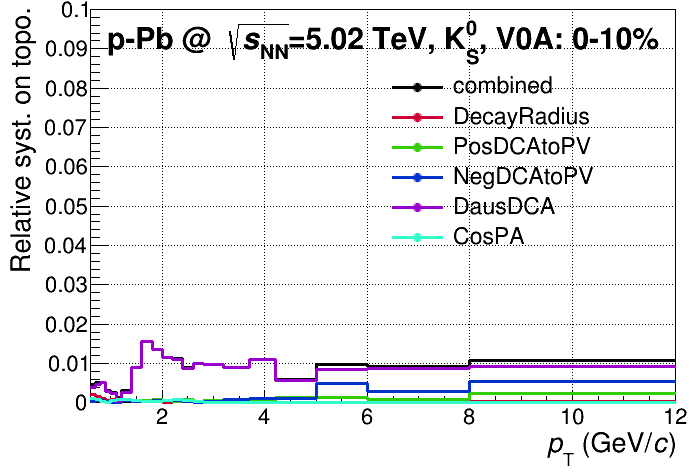
\includegraphics[width=.32\textwidth]{c06SystSelV0s/cKshort_MB_Syst_Topo_0}
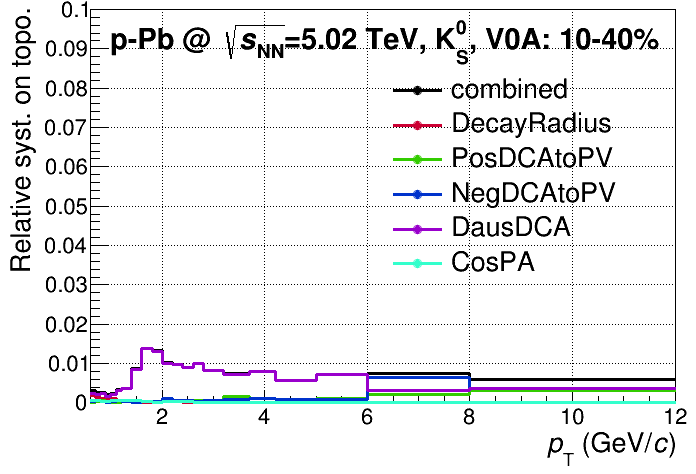
\includegraphics[width=.32\textwidth]{c06SystSelV0s/cKshort_MB_Syst_Topo_1}
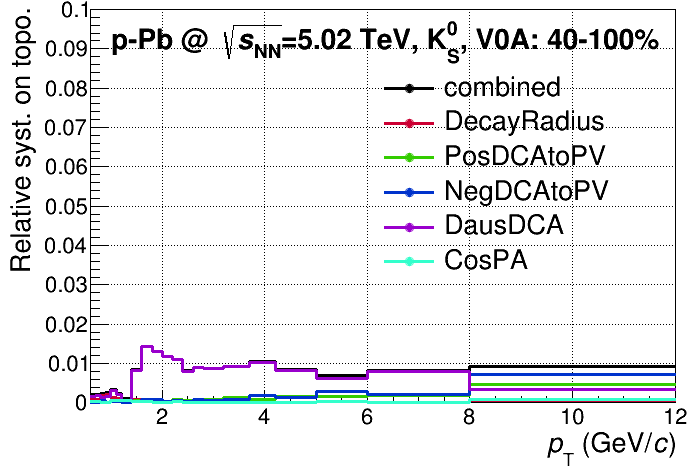
\includegraphics[width=.32\textwidth]{c06SystSelV0s/cKshort_MB_Syst_Topo_2}
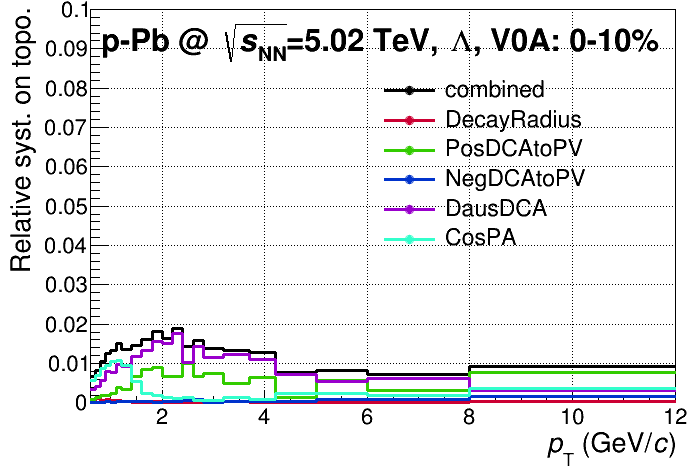
\includegraphics[width=.32\textwidth]{c06SystSelV0s/cLambda_MB_Syst_Topo_0}
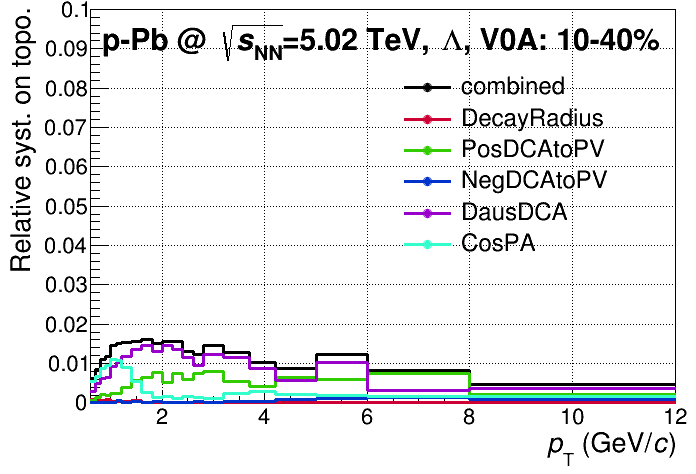
\includegraphics[width=.32\textwidth]{c06SystSelV0s/cLambda_MB_Syst_Topo_1}
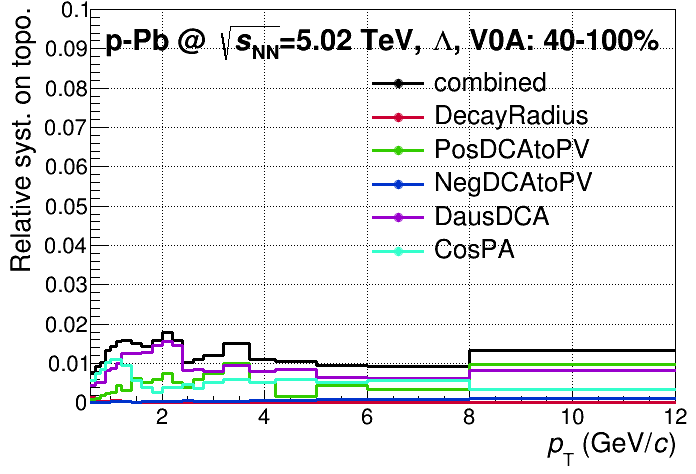
\includegraphics[width=.32\textwidth]{c06SystSelV0s/cLambda_MB_Syst_Topo_2}
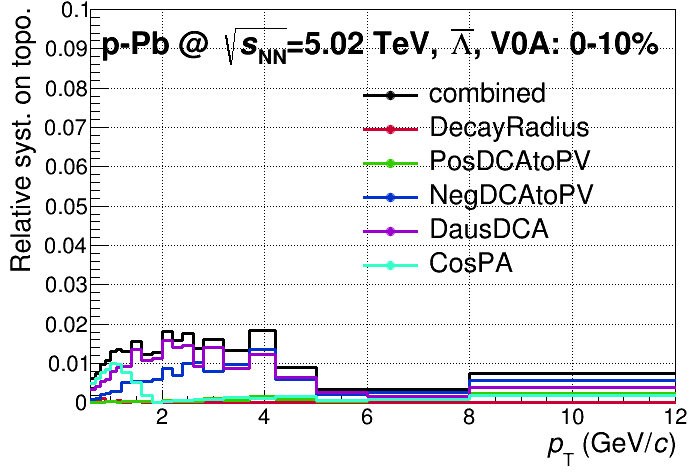
\includegraphics[width=.32\textwidth]{c06SystSelV0s/cAntiLa_MB_Syst_Topo_0}
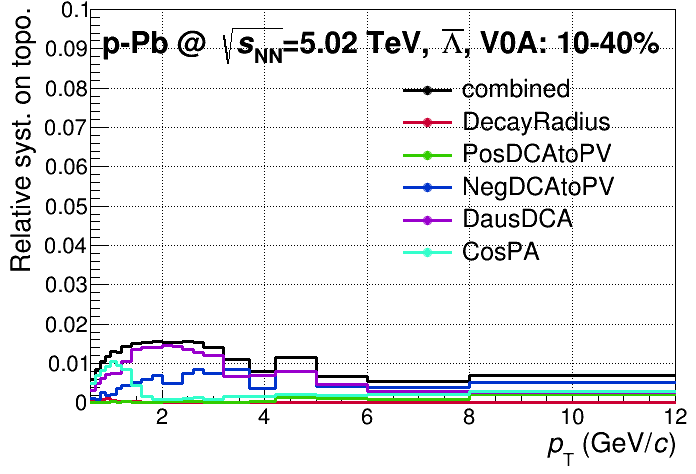
\includegraphics[width=.32\textwidth]{c06SystSelV0s/cAntiLa_MB_Syst_Topo_1}
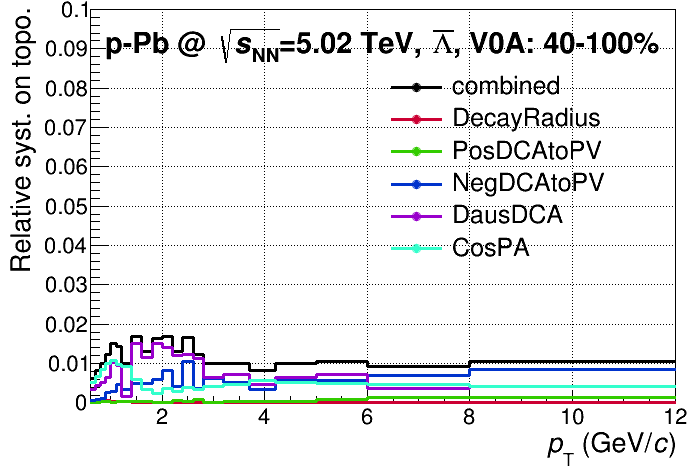
\includegraphics[width=.32\textwidth]{c06SystSelV0s/cAntiLa_MB_Syst_Topo_2}
\caption{Systematic uncertainty on topological selection as a function
         of $\pT$ in three event multiplicity bins with the V0A centrality
         estimator.}
\label{fig:c06SystTopo}
\end{center}
\end{figure}

\begin{figure}[htb]
\begin{center}
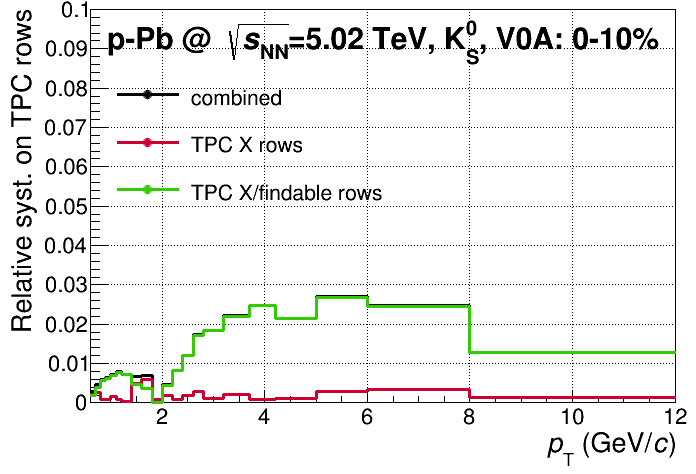
\includegraphics[width=.32\textwidth]{c06SystSelV0s/cKshort_MB_Syst_RowsTPC_0}
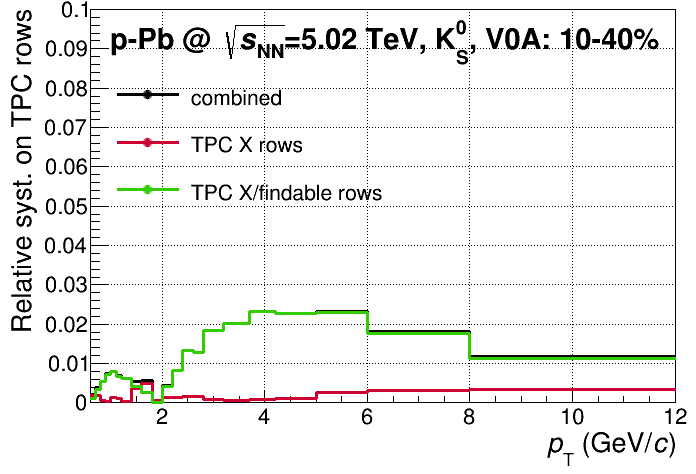
\includegraphics[width=.32\textwidth]{c06SystSelV0s/cKshort_MB_Syst_RowsTPC_1}
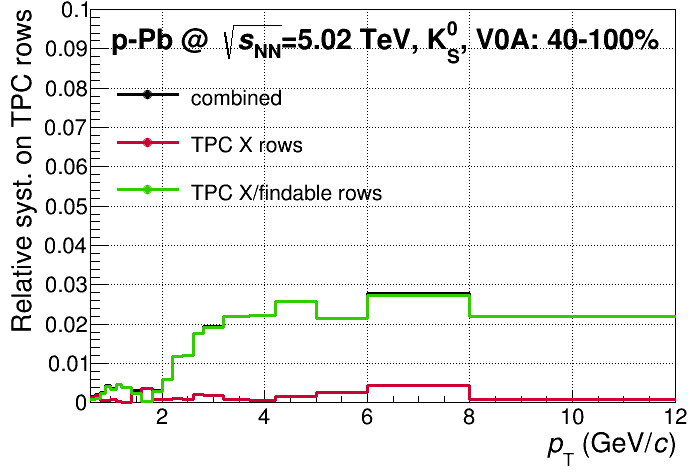
\includegraphics[width=.32\textwidth]{c06SystSelV0s/cKshort_MB_Syst_RowsTPC_2}
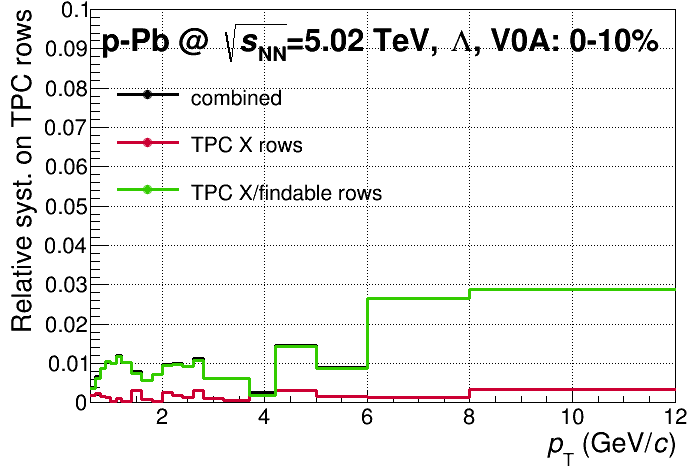
\includegraphics[width=.32\textwidth]{c06SystSelV0s/cLambda_MB_Syst_RowsTPC_0}
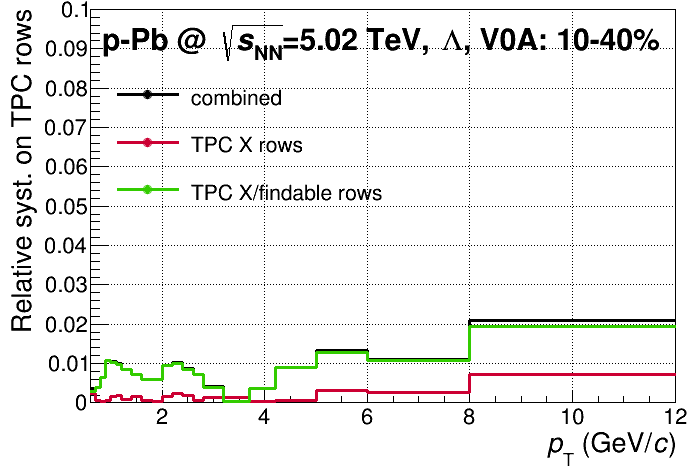
\includegraphics[width=.32\textwidth]{c06SystSelV0s/cLambda_MB_Syst_RowsTPC_1}
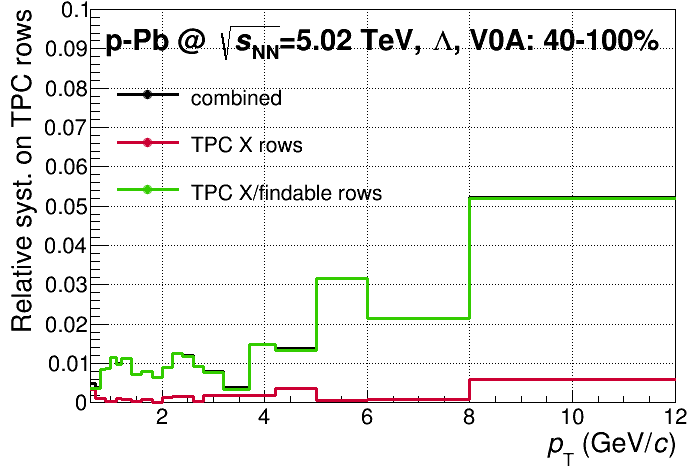
\includegraphics[width=.32\textwidth]{c06SystSelV0s/cLambda_MB_Syst_RowsTPC_2}
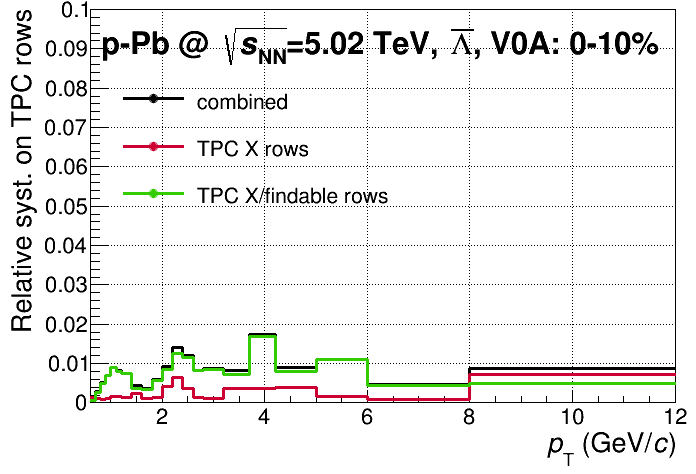
\includegraphics[width=.32\textwidth]{c06SystSelV0s/cAntiLa_MB_Syst_RowsTPC_0}
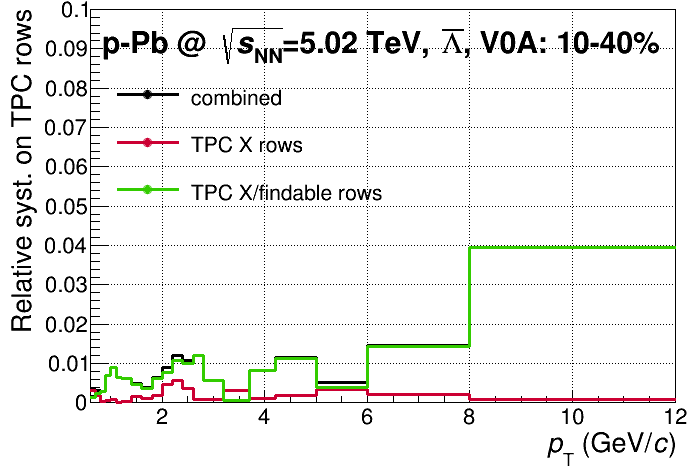
\includegraphics[width=.32\textwidth]{c06SystSelV0s/cAntiLa_MB_Syst_RowsTPC_1}
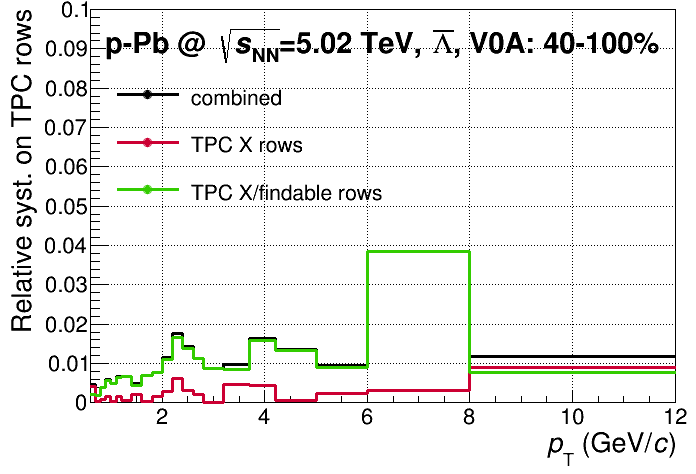
\includegraphics[width=.32\textwidth]{c06SystSelV0s/cAntiLa_MB_Syst_RowsTPC_2}
\caption{Systematic uncertainty on TPC rows selection for
         the $\Vzero$ daughter tracks. Results are shown as a function
         of $\pT$ and in three event multiplicity bins with the V0A
         centrality estimator.}
\label{fig:c06SystRowsTPC}
\end{center}
\end{figure}

\paragraph{Systematic uncertainty on $\Vzero$ candidate selection}
The systematic uncertainty on $\Vzero$ candidate selection is estimated
by varying the following cuts one by one in both data and MC.
\begin{itemize}
\item Topological selection:
      it is estimated by varying the topological variables listed
      in table~\ref{tab:c03ValSelV0Topo} with four additional different
      values as summarized in table~\ref{tab:c06TopoVars};
\item selections of proper lifetime, competing mass and
      TPC ${\rm d}E/{\rm d}x$ for $\Vzero$ daughter identification:
      the varied cut values for $\Kshort$ and $\Lambda$ ($\AntiLa$) are
      listed in table~\ref{tab:c06PropComp};
\item selection of the crossed TPC rows for $\Vzero$ daughters:
      it contains two set of cuts,
      the number of crossed TPC rows and the ratio between the number of
      crossed TPC row and the number of finable rows in TPC,
      the cut values are listed in table~\ref{tab:c06RowsTPC}.
\end{itemize}
For each of the cut,
the uncertainty is estimated by the maximum deviation between the results with
the varied cuts and that with the default cut (listed in
section~\ref{sec:c03V0CandiSel}).
The final uncertainty is given by quantitative sum of all the
uncertainty sources.

\begin{figure}[htb]
\begin{center}
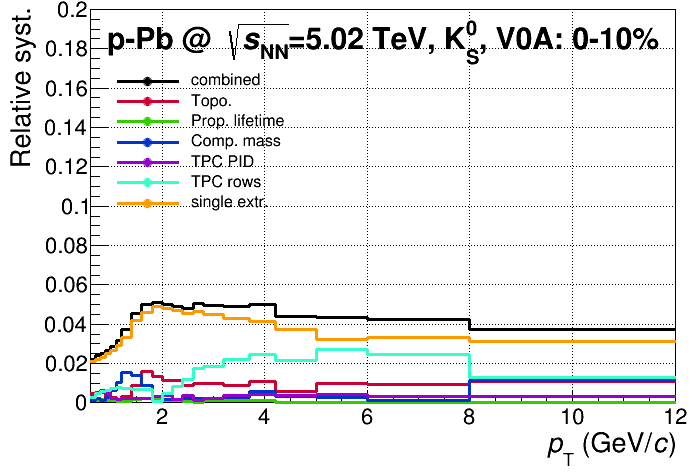
\includegraphics[width=.32\textwidth]{c06SystSelV0s/cKshort_MB_Syst_Total_0}
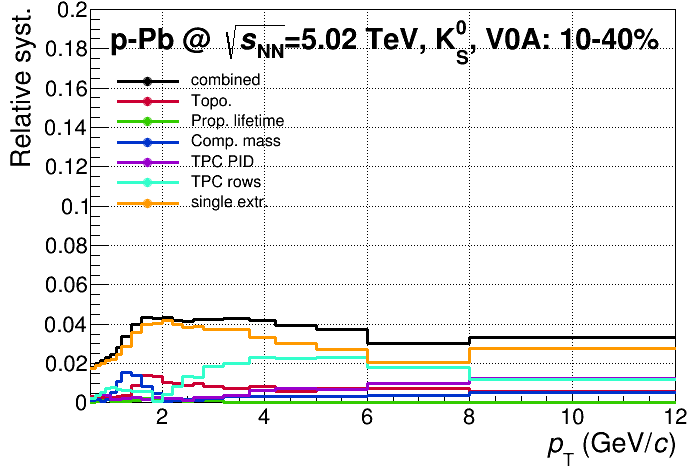
\includegraphics[width=.32\textwidth]{c06SystSelV0s/cKshort_MB_Syst_Total_1}
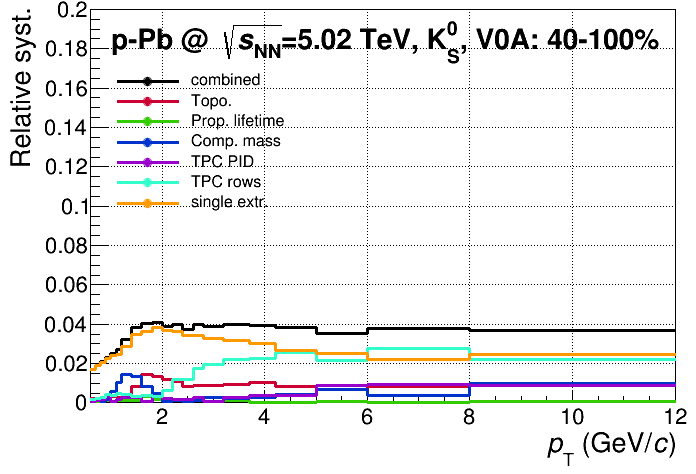
\includegraphics[width=.32\textwidth]{c06SystSelV0s/cKshort_MB_Syst_Total_2}
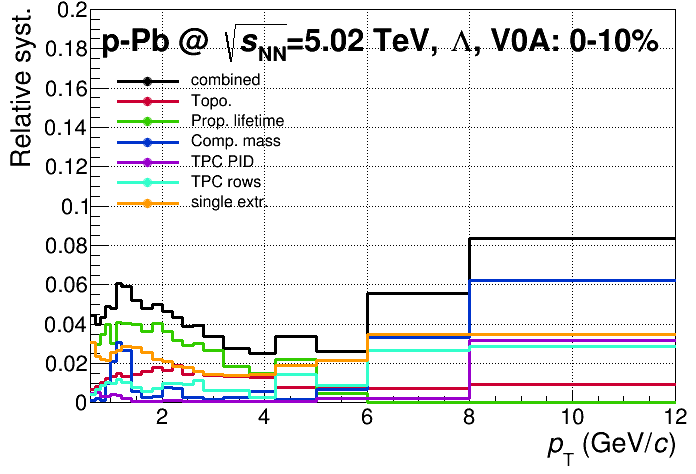
\includegraphics[width=.32\textwidth]{c06SystSelV0s/cLambda_MB_Syst_Total_0}
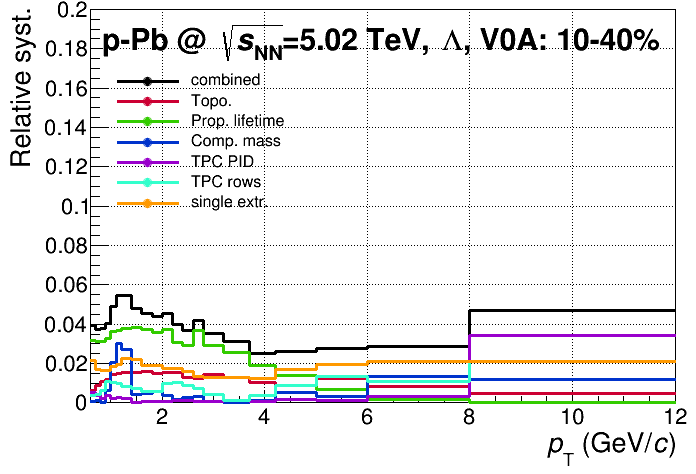
\includegraphics[width=.32\textwidth]{c06SystSelV0s/cLambda_MB_Syst_Total_1}
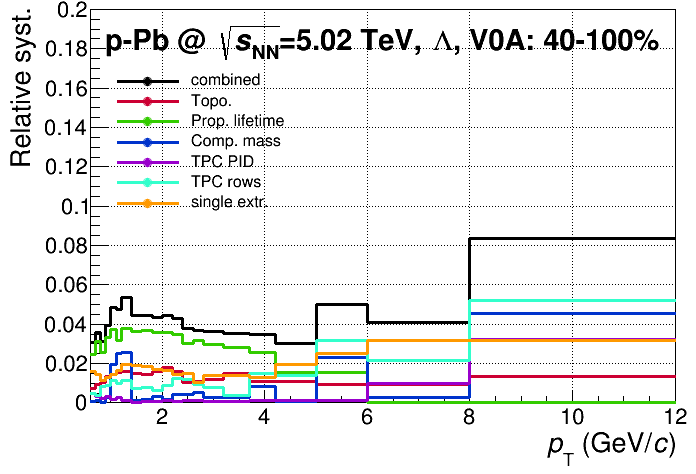
\includegraphics[width=.32\textwidth]{c06SystSelV0s/cLambda_MB_Syst_Total_2}
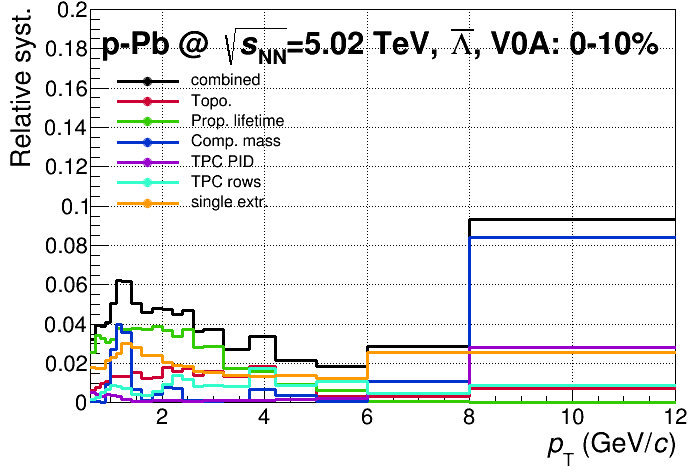
\includegraphics[width=.32\textwidth]{c06SystSelV0s/cAntiLa_MB_Syst_Total_0}
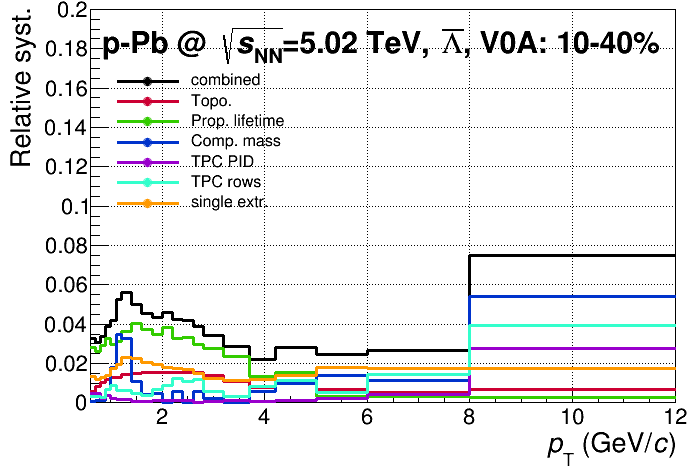
\includegraphics[width=.32\textwidth]{c06SystSelV0s/cAntiLa_MB_Syst_Total_1}
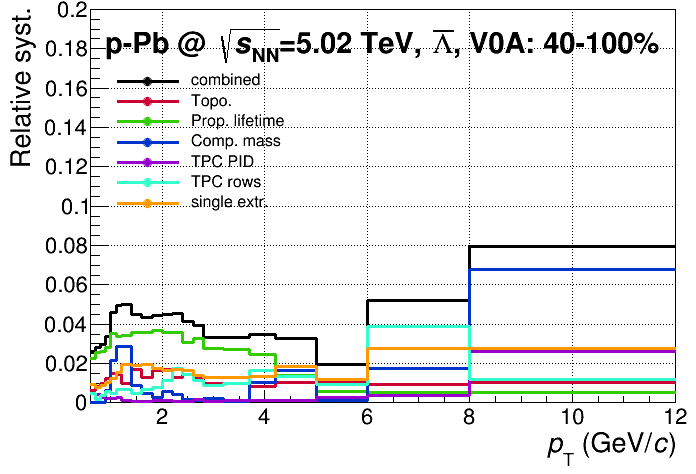
\includegraphics[width=.32\textwidth]{c06SystSelV0s/cAntiLa_MB_Syst_Total_2}
\caption{Uncertainties on $\Vzeros$ candidates selection and $\Vzero$ signal
         extraction.
         The results are shown as a function of $\pT$ and in three event
         multiplicity bins with the V0A centrality estimator.
         The combined uncertainty are the quantitative sum of all the sources.}
\label{fig:c06SystTotal}
\end{center}
\end{figure}

\paragraph{Systematic uncertainty on $\Vzero$ signal extraction}
As mentioned in section~\ref{sec:c03AnaStrategy},
the number of $\Vzero$ signals is extracted in the window defined
in $N\sigma$ after subtracting the interpolated bin counting fit result.
The default value to build the signal window is $N=5$.
The uncertainty on $\Vzero$ signal extraction is given by $N=4,~6~{\rm and}~7$.
The value of $N$ is also changed simultaneously in both data and MC.
The systematic uncertainty is estimated as the maximum deviation between
the results with varied $N$ values and that with $N=5$.

\paragraph{Relative uncertainty of inclusive $\Vzeros$}
Figures~\ref{fig:c06SystTopo} shows the uncertainty on topological selection
for different variables.
The results are shown as a function of $\pT$ and in three event multiplicity
bins with the V0A centrality estimator.
The combined results are the quantitative sum of all the sources.
In general, the uncertainty on the topological selection varies
from $2\%$ to $1\%$ from low to high $\pT$.
For both $\Kshort$ and $\Lambda$ ($\AntiLa$) the uncertainty is dominated
by the uncertainty on the DCA between the daughter tracks.
But the contribution from the uncertainty on $\cos\theta_{\rm pointing}$
becomes important in the hight $\pT$ region for $\Lambda$ ($\AntiLa$).
The uncertainty on TPC rows selection are shown
in figure~\ref{fig:c06SystRowsTPC}.
In all of the cases, the uncertainty on number of crossed TPC rows is
small ($<1\%$).
But the uncertainty on the ratio of number of crossed rows and findable
rows in TPC is much larger.
In general, it has the order of $\mathcal{O}(2\%)$ and
it achieves to $3\%-5\%$ in some cases,
especially in hight $\pT$ region.
 
 The systematical uncertainties on the $\Vzero$ candidates selection
and $\Vzero$ signal extraction are compared in figure~\ref{fig:c06SystTotal}.
The combined uncertainty is the quantitative sum of all the sources.
For $\Kshort$, the combined uncertainty is dominated by the uncertainty on
signal extraction,
And the contribution from the TPC rows selection becomes important
in high $\pT$ region.
For $\Lambda$ and $\AntiLa$, the combined uncertainty is mainly contributed
by the uncertainty on proper lifetime selection in low $\pT$ region,
and in high $\pT$ the uncertainty is dominated by the uncertainty on the
competing mass selection since this cut has been removed to estimate the
corresponding uncertainty for $\Lambda$ and $\AntiLa$.

\paragraph{Uncertainty of the JC and UE $\Vzeros$}
The different uncertainty sources on the single $\Vzero$ analysis of the
inclusive $\Vzeros$ are summarized in figure~\ref{fig:c06SystTotal}.
Since the $\Vzeros$ and jets are reconstructed independently in this analysis,
the uncertainty on the $\Vzero$ candidate selection and that on the material
budget of the inclusive $\Vzeros$ should be the same as those of the JC
and UE $\Vzeros$.
In particular, the statistics of the inclusive $\Vzeros$ is much higher
than the the JC or UE $\Vzeros$,
the correlations between the systematic uncertainty on the $\Vzero$ candidates
selection estimated by using the inclusive $\Vzeros$ and the statistics is week.

For the uncertainty on $\Vzero$ single extraction,
since it contains the uncertainty on the bin counting
fit which depends on the statistics.
In this case,
we reproduced the procedures used to estimate the uncertainty
on $\Vzero$ signal extraction to the JC and UE $\Vzeros$.
This uncertainty is estimated
as $6\%$ with $\pT^{\rm jet}>10~\GeVc$ and $10\%$ with
$\pT^{\rm jet}>20~\GeVc$ independent with the $\Vzero$ $\pT$.

\paragraph{Discussion}
In section~\ref{sec:c05ScaledV0Effi},
to obtain the $\eta$ modified $\Vzero$
efficiency (the eq.~(\ref{eq:c05CorrEffImp})),
we assume that, the bin counting ratio (the $R_{\rm Cbin}$ defined
in eq.~(\ref{eq:c03CbinR}))
in the integrated $\eta$ region and in each sub-$\eta$ region is the same in
both data and MC.
Indeed, this ratio should be changed between the fine $\eta$ bins
due to the acceptance of the $\Vzero$ daughter
tracks (the bin counting ratio in the $\eta$ region towards to the bound of
the daughter track acceptance should be different from that in the rest ones).
Here, we claim that,
the uncertainty introduced by this assumption is included in the
uncertainty on single $\Vzero$ analysis, because of the following reasons:
\begin{itemize}
\item the contribution in the $\eta$ region towards to the bound of the
      daughter track acceptance is small in the final result;
\item the bin counting ratio will be changed if we varying the cuts of
      the $\Vzero$ daughter track selection and $\Vzero$ topological
      selection to estimate the uncertainty on $\Vzero$ candidate selection;
\item when we varying the signal window and slide bands to the estimate
      the uncertainty on $\Vzero$ signal extraction,
      it also changes the bin counting ratio since the inputs for the bin
      counting fit have been changed.
\end{itemize}
In this case, the fluctuations of the bin counting ratio between the
fine $\eta$ bins will be contained in the uncertainty on the
single $\Vzero$ analysis.

\subsubsection{Uncertainty on underlying $\Vzero$ subtraction}

\begin{figure}[htb]
\begin{center}
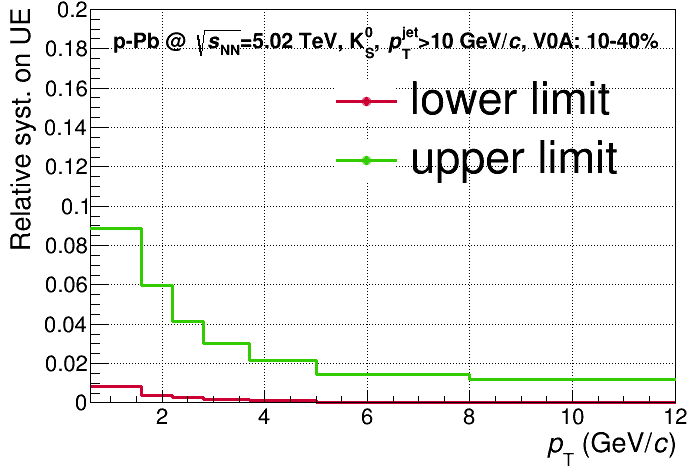
\includegraphics[width=.32\textwidth]{c06SystUE/cKshort_Syst_UE_1}
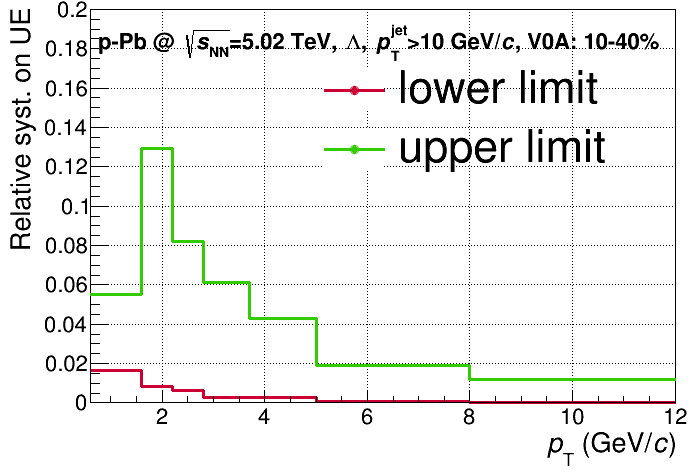
\includegraphics[width=.32\textwidth]{c06SystUE/cLambda_Syst_UE_1}
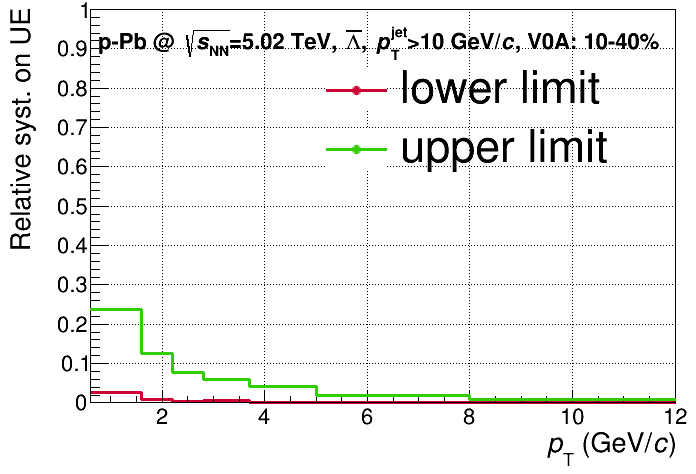
\includegraphics[width=.32\textwidth]{c06SystUE/cAntiLa_Syst_UE_1}
\caption{The relative systematic uncertainty on underlying $\Vzero$ subtraction.
The results are shown in $10-40\%$ event multiplicity bin.
The upper and lower uncertainty bands are shown in green and red, respectively.}
\label{fig:c06SystUE}
\end{center}
\end{figure}

As mentioned in section~\ref{sec:c05EstiV0sUE},
the underlying $\Vzeros$ are estimated by two approached:
the OC $\Vzeros$ and the NJ $\Vzeros$.
According to the discussion in section~\ref{sec:c05NormResults},
the spectrum of OC $\Vzeros$ is harder than that of the NJ $\Vzeros$.
And for the OC $\Vzeros$, the normalized spectrum built with the
smaller $\Delta R_{\rm cut}$ is higher than those build with the
larger $\Delta R_{\rm cut}$.
To estimate the uncertainty on underlying $\Vzero$ subtraction,
we use the OC $\Vzeros$ with $\Delta R_{\rm cut}=0.6$ to build the
centre value of the spectrum for the $\Vzeros$ produced inside jet:
\begin{equation}
{\rm JE}={\rm JC}-{\rm OC}(\Delta R_{\rm cut}=0.6),
\end{equation}
 and use the OC $\Vzeros$ with $\Delta R_{\rm cut}=0.4$ and
NJ $\Vzeros$ to build the asymmetry band:
\begin{equation}\label{eq:c06BandUE}
[{\rm JC}-{\rm OC}(\Delta R_{\rm cut}=0.4), {\rm JC}-{\rm NJ}].
\end{equation}

The band defined in eq.~(\ref{eq:c06BandUE}) gives region where the spectra
of the $\Vzeros$ produced inside the jets is located and it is not equal to
the RMS which is generally used to define the uncertainty.
By following the strategy in~\cite{Ali2013:ana921},
we assume the distribution of JE $\Vzeros$ is uniform~\footnote{As discussed
in~\cite{Ali2013:ana921}, the advantage to assume the uniform distribution
in the band is that,
it can minimize the bias introduced by the assumption of the distribution
for the uncertainty estimation as well as to minimize the correlations
between the other uncertainty sources.}
in the band defined
in eq.~(\ref{eq:c06BandUE}), then the RMS of the band is given by:
\begin{equation}\label{eq:c06UEbandRMS}
[\frac{{\rm JC}-{\rm OC}(\Delta R_{\rm cut}=0.4)}{\sqrt{12}},
\frac{{\rm JC}-{\rm NJ}}{\sqrt{12}}].
\end{equation}

The eq.~(\ref{eq:c06UEbandRMS}) is used to give the uncertainty on the underlying $\Vzero$ subtraction on the $\pT$ spectrum.
As an example,
the relative systematic uncertainty on underlying $\Vzero$
subtraction in $10-40\%$ event multiplicity bin is presented
in figure~\ref{fig:c06SystUE}.
The upper and lower bands in eq.~(\ref{eq:c06UEbandRMS}) are shown
in green and red, respectively.
The lower limit of the uncertainty is awayls small.
For the upper limit, it arises to $\sim 10\%$ in low $\pT$ region,
then it decreases to a few percent in the high $\pT$ region as expected.
In principle, the uncertainty for $\Lambda$ and $\AntiLa$ should be
very similar.
But figure~\ref{fig:c06SystUE} shows a large difference of the upper limit
of the uncertainty between $\Lambda$ and $\AntiLa$ in the low $\pT$ region.
This could be caused by the UE $\Vzeros$ is dominated in the low $\pT$ and
the uncertainty on UE $\Vzero$ subtraction is more sensitive to the
statistic fluctuations than that in the high $\pT$ region.

\begin{figure}[htb]
\begin{center}
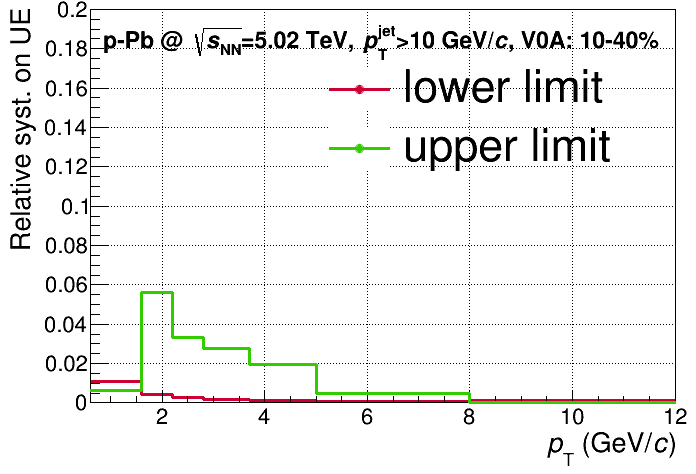
\includegraphics[width=.8\textwidth]{c06SystUE/cRatioV_Syst_UE_1}
\caption{The relative systematic uncertainty on underlying $\Vzero$
         subtraction for the $\Kshort$-to-$\Lambda$ ratio.
         The results are shown in $10-40\%$ event multiplicity bin.
         The upper and lower uncertainty bands are shown in green and red,
         respectively.}
\label{fig:c06SystRatioVUE}
\end{center}
\end{figure}

Since the OC and NJ $\Vzeros$ are correlated with the jet $\pT$ which used to
define the OC and NJ events,
to calculate the uncertainty on underlying $\Vzero$ subtraction for the
$\Kshort$-to-$\Lambda$ ratio we did not propagate them from the uncertainty
on the $\Vzero$ spectrum directly but use the following steps:
\begin{itemize}
\item calculate the $\Kshort$-to-$\Lambda$ ratio ($R_{{\rm K}/\Lambda}$) with
      varies UE $\Vzeros$;
\item the centre value is given by using the OC $\Vzeros$
      with $R_{\rm cut}=0.6$:
      \begin{equation}
      R_{{\rm K}/\Lambda}({\rm JC}-{\rm OC}_{R_{\rm cut}=0.6});
      \end{equation}
\item the upper and lower limits of the uncertainty are given by:
      \begin{equation}\label{eq:c06SystUERatioV}
      [\frac{R_{{\rm K}/\Lambda}({\rm JC}-{\rm OC}_
            {R_{\rm cut}=0.4})}{\sqrt{12}},
       \frac{R_{{\rm K}/\Lambda}({\rm JC}-{\rm NJ})}{\sqrt{12}}].
      \end{equation}
\end{itemize}
As an example, figure~\ref{fig:c06SystRatioVUE} shows one of uncertainty
results for the $\Kshort$-to-$\Lambda$ ratio.

\subsubsection{Uncertainty on feeddown subtraction}
\label{sec:c06SystFd}

\begin{figure}[htb]
\begin{center}
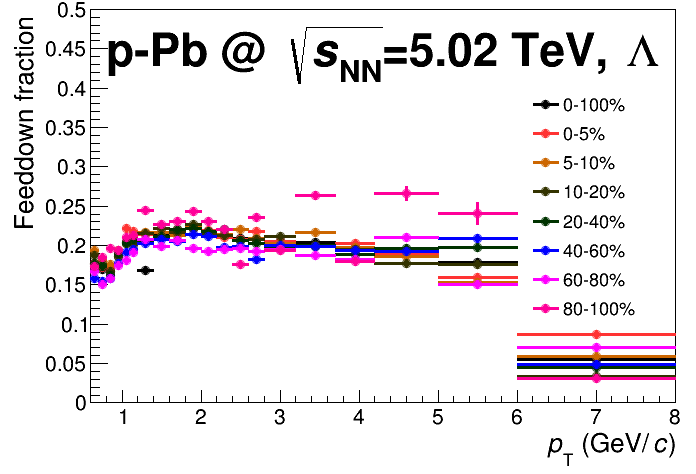
\includegraphics[width=.49\textwidth]{c06Feeddown/cLambda_Fraction_FD}
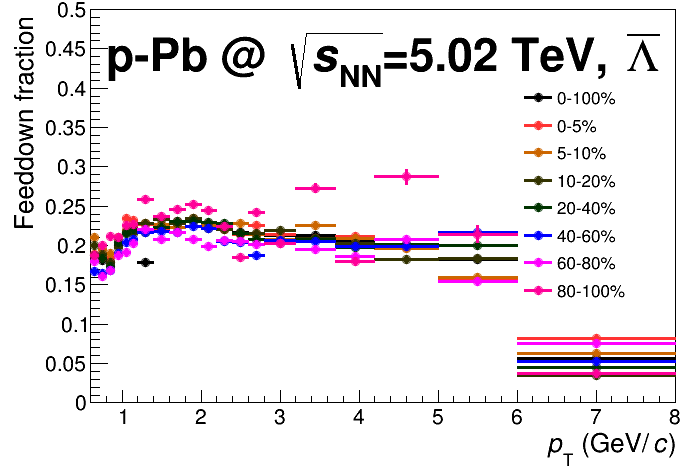
\includegraphics[width=.49\textwidth]{c06Feeddown/cAntiLa_Fraction_FD}
\caption{Feeddown fraction of inclusive $\Lambda$ (left) and $\AntiLa$ (right)
         from $\Xi$ decays obtained in data.}
\label{fig:c05FractionFd}
\end{center}
\end{figure}

\begin{figure}[htb]
\begin{center}
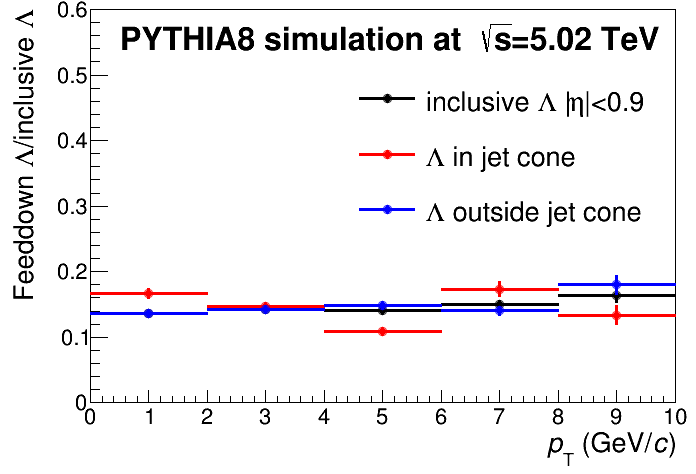
\includegraphics[width=.49\textwidth]{c06Feeddown/chLaRatio}
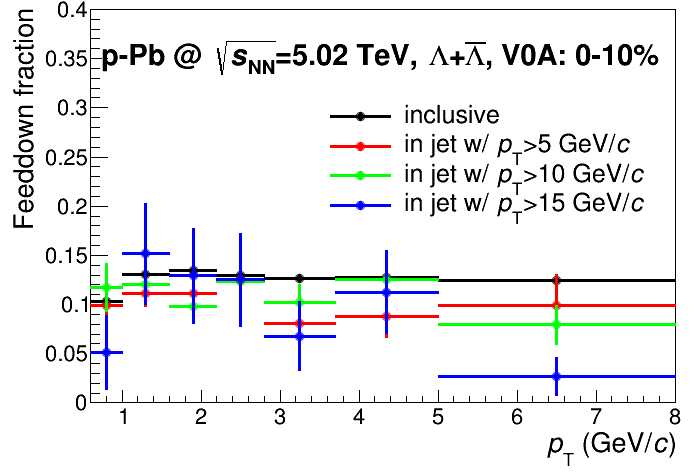
\includegraphics[width=.49\textwidth]{c06Feeddown/cLaFeeddown}
\caption{Feeddown fraction of inclusive $\Lambda$ ($\AntiLa$) from PYTHIA8
         simulations (left) and from the DPMjet simulations (right).
         The results from PYTHIA8 simulation is obtained at particle level and
         results from DPMjet simulations is obtained from the detector level.}
\label{fig:c05FractionFdSim}
\end{center}
\end{figure}

The uncertainty on feedddown subtraction (for $\Lambda$ and $\AntiLa$) in
the inclusive $\Vzero$ spectrum is from the uncertainty on $\Xi$ measurement
and the feeddown production
extrapolation (in hight $\pT$)~\cite{Ali2012:ana501,Ali2013:ana702}.
The value varies from $5\%$ (in $\pT<3.7~\GeVc$)
to $7\%$ (in $\pT>3.7~\GeVc$)~\cite{Ali2013:ana702}.

To correct the feeddown for the $\Vzeros$ inside jets,
one has to consider the production of $\Xi$ inside jets could be
different from that of the inclusive one.
And it will make difference between the feeddown fraction of the
inclusive $\Vzeros$ and $\Vzeros$ produced inside jets.

Since there is no $\Xi$ data measured in jets,
a conservative scenario was applied to estimate the uncertainty on
feeddown correction in this analysis.

Figure~\ref{fig:c05FractionFdSim} shows the feeddown fraction of $\Vzeros$ in
jets and the inclusive $\Vzeros$ from the PYTHIA8 (left) and DPMjet
simulations (right).
The results from PYTHIA8 simulation is obtained at particle level and
results from DPMjet simulations is obtained from the detector level.
In both PYHTIA and DPMjet, it shows that, the feeddown fraction for both
inclusive $\Vzeros$ and $\Vzeros$ in jets are very similar, $\sim 10\%$,
and the results are insensitive to the $\pT$ of $\Vzeros$ and jets.
While in data, as shown in figure~\ref{fig:c05FractionFd},
the feeddown fraction of inclusive $\Vzero$ shows a week $\pT$-dependence
and it is $\sim 20\%$ at low and intermedia-$\pT$.

\begin{figure}[htb]
\begin{center}
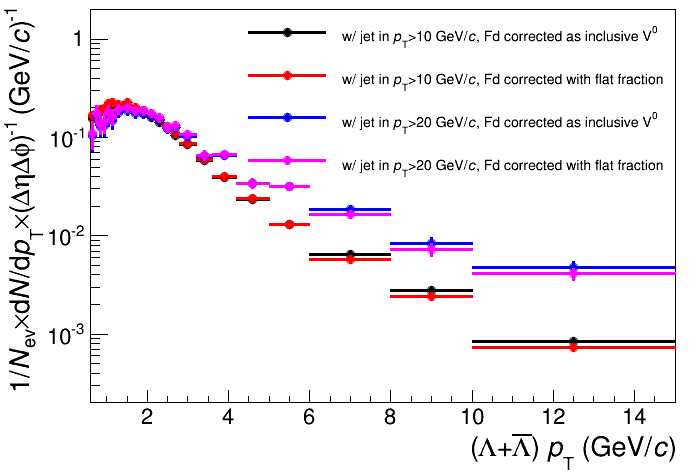
\includegraphics[width=.49\textwidth]{c06Feeddown/cCompLa}
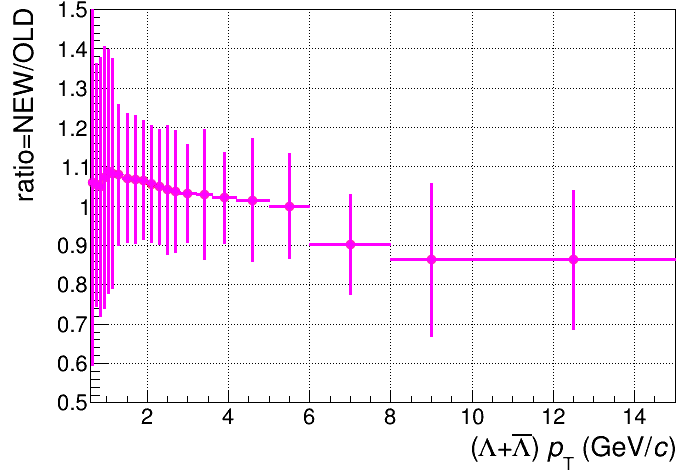
\includegraphics[width=.49\textwidth]{c06Feeddown/cCompLa_Ratio}
\caption{Right: the spectra of JC $\Lambda+\AntiLa$ after the feeddown
         subtraction with different feeddown fraction templates.
         Left: the ratio between the $\Lambda+\AntiLa$ spectra with
         different feeddown subtraction templates.}
\label{fig:c05CompFd}
\end{center}
\end{figure}

According to these studies, we subtract the feeddown component of
the $\Vzeros$ in jets by using the feeddown fraction of the
inclusive $\Vzeros$ and a const feeddown fraction as $10\%$, respectively.
The uncertainty on the feeddown subtraction is estimated by using the
deviation between the results with these two feeddown templates.
Figure~\ref{fig:c05CompFd} shows the feeddown subtracted
spectra of $\Lambda+\AntiLa$ with different feeddown fraction
templates (right) and the ratio between them (left).
A maximum $10\%$ deviation is found in the results.
In the final results, we used the mean given by these two feeddown fraction
templates as the centre value of the spectrum for the $\Vzeros$ produced
in jets and added and additional $5\%$ uncertainty to the uncertainty on
feeddown correction for the inclusive $\Vzeros$.

\subsubsection{Uncertainty on jet $\pT$}

\begin{figure}[htb]
\begin{center}
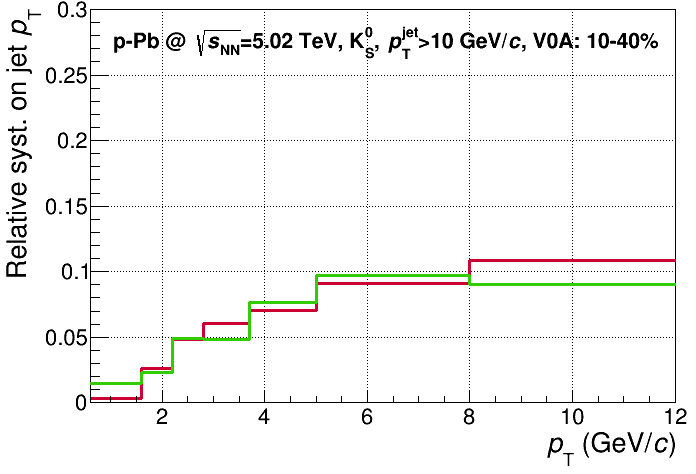
\includegraphics[width=.32\textwidth]{c06SystPtJ/cKshort_Syst_PtJ_1}
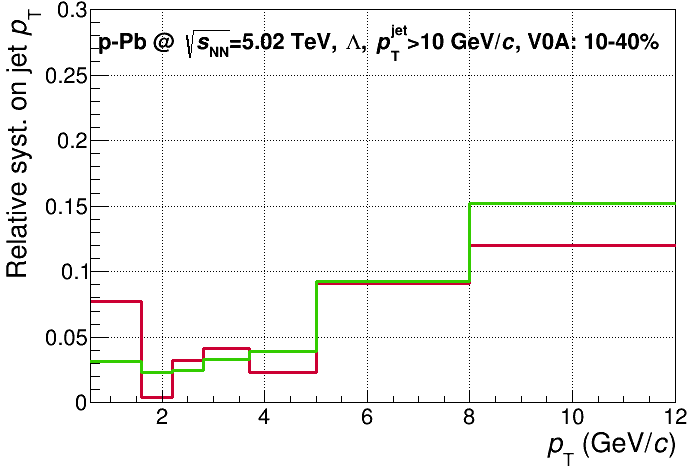
\includegraphics[width=.32\textwidth]{c06SystPtJ/cLambda_Syst_PtJ_1}
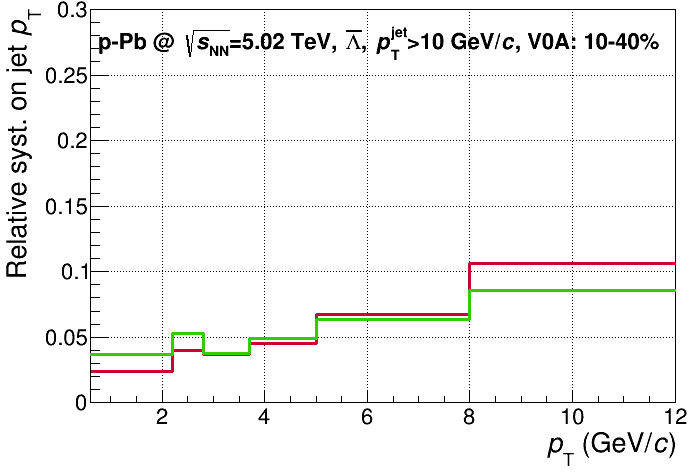
\includegraphics[width=.32\textwidth]{c06SystPtJ/cAntiLa_Syst_PtJ_1}
\caption{The relative systematic uncertainty on jet $\pT$ scale.
         The results are shown in $10-40\%$ event multiplicity bin.
         The upper and lower uncertainty bands are shown in green and red,
         respectively.}
\label{fig:c06SystPtJ}
\end{center}
\end{figure}

Indeed, in this analysis, we have to correct both of the reconstructed and
acceptance efficiency of $\Vzeros$ and the $\pT$ of the jets.
For the jet $\pT$, the correction includes the one for the background
fluctuations and that for the detector response.
In the analysis of the inclusive jet spectra,
this correction is applied via an unfolding approach~\cite{Ali2012:ana58}.
By considering the $\Vzero$ productions inside the jets,
the $\pT$ of $\Vzeros$ is correlated with the jet $\pT$.
And a $2$-dimension has to be applied in this analysis.
We tried this 2D in our earlier analysis~\cite{zhang:AliPWGJE20130920},
but it is hard to build a stable result due to the less of the statistics.

Alternatively, a bin-by-bin  approach has been proposed to correct spectra of
particles produced in jets~\cite{Ali2012:ana067}.
With this method, the reconstruction and acceptance efficiency of $\Vzeros$,
the jet background fluctuations and the detector response of jet $\pT$ will
be corrected synchronously.
According to the discussion is section~\ref{sec:c05ScaledV0Effi},
the efficiency of $\Vzeros$ in jets is depend on the jet
modified $\Vzero$ $\eta$ distribution.
Since the MC can neither reproduce the distribution of $\Vzeros$ nor the
distribution of jets,
the $\Vzero$ efficiency calculation should be separated from the
bin-by-bin correction.
Also, the jet background fluctuations are not well described in MC,
even the jet background density in p--Pb collisions is much smaller than
that in Pb--Pb collisions.

In this analysis, we calculate the $\Vzero$ efficiency via the scaling
approach as introduced in section~\ref{sec:c05ScaledV0Effi} and treat the
effect of the jet background fluctuations and the detector response effect
on jet $\pT$ as the systematic uncertainty.

\begin{figure}[htb]
\begin{center}
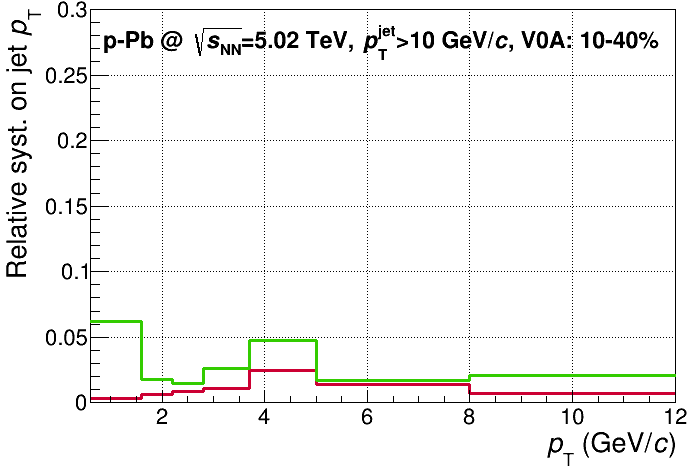
\includegraphics[width=.8\textwidth]{c06SystPtJ/cRatioV_Syst_PtJ_1}
\caption{The relative systematic uncertainty on jet $\pT$ scale
         in  $\Kshort$-to-$\Lambda$ ratio.
         The results are shown in $10-40\%$ event multiplicity bin.
         The upper and lower uncertainty bands are shown in green and red,
         respectively.}
\label{fig:c06SystRatioVPtJ}
\end{center}
\end{figure}

\paragraph{Systematic uncertainty on jet background fluctuations}
The systematic uncertainty on jet background fluctuations is estimated by
varying the jet $\pT$ threshold
in $20\%$~\footnote{The uncertainty of $\Vzeros$ in jets with $\pT>10~\GeVc$
is estimated by varying the jet $\pT$ threshold from $8$ to $12~\GeVc$.
And the uncertainty of $\Vzeros$ in jets with $\pT>20~\GeVc$
is estimated by varying the jet $\pT$ threshold from $16$ to $24~\GeVc$.}
Since the RMS in of the $\delta\pT$ distribution (as shown
in figure~\ref{fig:c04DeltapT}) is $\sim 1~\GeVc$,
the jet background fluctuations should be included in the band built by
varying the jet $\pT$ in $20\%$ safely.
The same as the estimation for the uncertainty on underlying event subtraction,
we assume the distribution of the JE $\Vzeros$ in the band built by the upper
and lower jet $\pT$ threshold is uniform and give the upper and lower limits
of the uncertainty as:
\begin{equation}
[\frac{{\rm JE}(\pT^{\rm jet}>(1-20\%)\pT^{\min})}{\sqrt{12}},
 \frac{{\rm JE}(\pT^{\rm jet}>(1+20\%)\pT^{\min})}{\sqrt{12}}].
\end{equation}
Due to the production of UE $\Vzeros$ is correlated with the
jet $\pT$ threshold,
the same approach as defined in eq.~(\ref{eq:c06SystUERatioV}) is used to
estimate the uncertainty in the $\Kshort$-to-$\Lambda$ ratio:
\begin{equation}
[\frac{R_{{\rm K}/\Lambda}^{\rm JE}(\pT^{\rm jet}>(1-20\%)\pT^{\min})}
      {\sqrt{12}},
 \frac{R_{{\rm K}/\Lambda}^{\rm JE}(\pT^{\rm jet}>(1+20\%)\pT^{\min})}
      {\sqrt{12}}].
\end{equation}

As an example,
the relative uncertainty on jet background fluctuations in the $\Vzero$ spectra
and that in the $\Kshort$-to-$\Lambda$ are shown in
figure~\ref{fig:c06SystPtJ} and
figure~\ref{fig:c06SystRatioVPtJ}, respectively.
The results are shown in $10-40\%$ event multiplicity bin.
The upper and lower uncertainty bands are shown in green and red, respectively.
The uncertainty in the $\Vzero$ spectrum increases with the $\Vzero$ $\pT$.
While the uncertainty in the $\Kshort$-to-$\Lambda$ is insensitive to the $\pT$.

\begin{figure}[htb]
\begin{center}
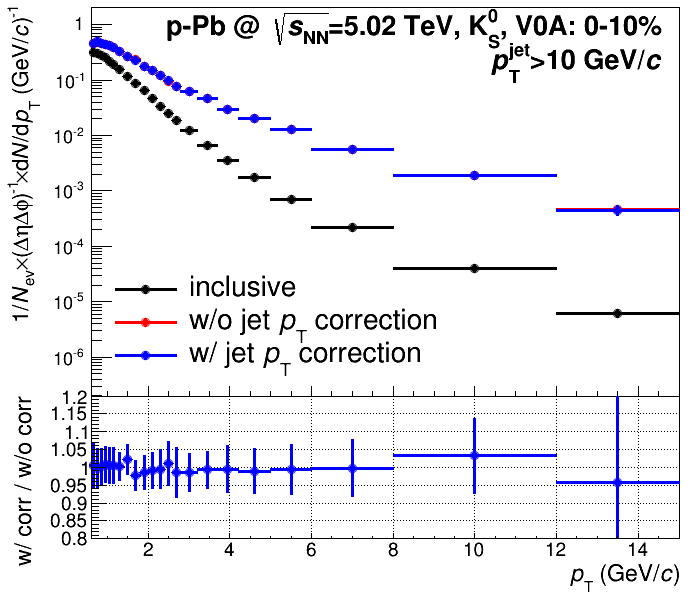
\includegraphics[width=.32\textwidth]{c06SystPtJ/cKshort_CorrPtJ}
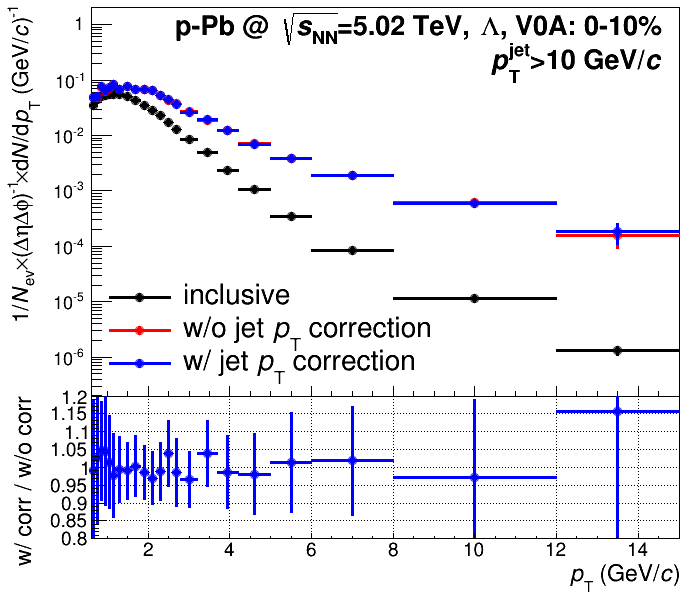
\includegraphics[width=.32\textwidth]{c06SystPtJ/cLambda_CorrPtJ}
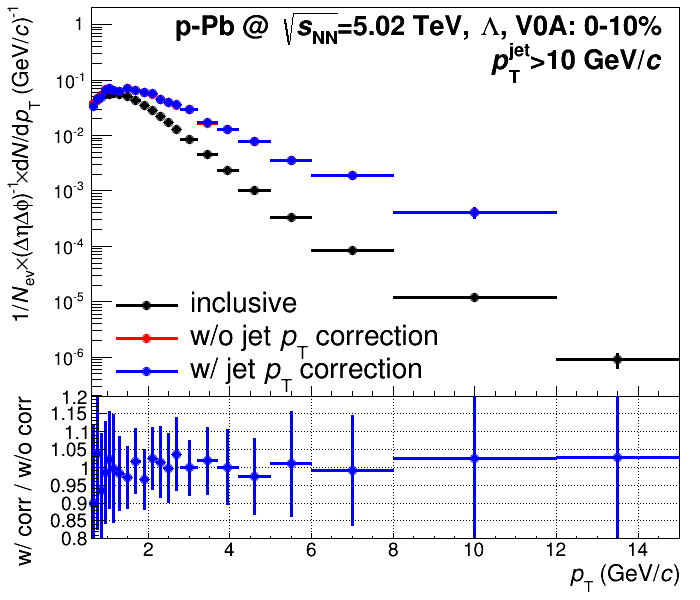
\includegraphics[width=.32\textwidth]{c06SystPtJ/cAntiLa_CorrPtJ}
\caption{The comparison of the spectrum of $\Vzeros$ produced in jets with
         detector response corrected jet $\pT$ and that without the detector
         response correction.}
\label{fig:c06SystDetResp}
\end{center}
\end{figure}

\paragraph{Uncertainty on detector response}
The detector response matrix (as shown in figure~\ref{fig:c04DetectorRM})
describes the effect of the  single track efficiency in the reconstructed
jet $\pT$.
The following steps are used to check this effect in the $\Vzero$ productions
in jets:
\begin{enumerate}
\item smear the background subtracted jet $\pT$ in data with the response
      matrix and recover it to the particle level;
\item apply the cut on the smeared jet $\pT$ and redo the analysis to get
      the $\Vzero$ production in jets.
\end{enumerate}
A comparison of the spectrum of $\Vzeros$ produced in jets with detector
response corrected jet $\pT$ and that without the detector response
correction is shown in figure~\ref{fig:c06SystDetResp}.
The difference between the results with and without the detector response
correction is very small.
This testing is quite similar as the bin-by-bin correction if only the
detector response is considered.
In this case, we only use the uncertainty given by varying the
jet $\pT$ threshold within $20\%$ as the uncertainty on jet $\pT$ scale.
